\documentclass[tikz,border=8pt]{standalone}
% Shared look for every TikZ diagram. Load with \input{../../tools/tikz-style.tex}
\usepackage[sfdefault]{roboto}
\usetikzlibrary{arrows.meta, positioning, shapes.geometric, calc, fit, backgrounds}
\definecolor{cblue}{HTML}{4C78A8}
\definecolor{corange}{HTML}{F58518}
\definecolor{cgreen}{HTML}{54A24B}
\definecolor{cred}{HTML}{E45756}
\definecolor{cpurple}{HTML}{B279A2}
\definecolor{cgrey}{HTML}{6B6B6B}
\tikzset{
  every picture/.style={font=\sffamily, line width=1.2pt},
  box/.style={draw=#1, fill=#1!12, rounded corners=4pt, align=center, inner sep=7pt, minimum height=1.1cm},
  box/.default=cgrey,
  arrow/.style={-{Stealth[length=3mm]}, draw=cgrey, line width=1.4pt},
  title/.style={font=\sffamily\bfseries\Large},
  note/.style={font=\sffamily\small, text=cgrey, align=center},
}
\AtBeginDocument{\hyphenpenalty=10000 \exhyphenpenalty=10000}

% Autoware's behaviour path planner (autowarefoundation/autoware_universe, main, read 2026-10-12).
% Top: the four slots of config/scene_module_manager.param.yaml; each slot takes the path from the one before.
% Bottom left: a scene module's states (scene_module_interface.hpp, updateState()).
% Bottom right: the two stacks of one slot (docs/behavior_path_planner_manager_design.md), on the design
% document's example of avoiding a parked car during a lane change.
\begin{document}
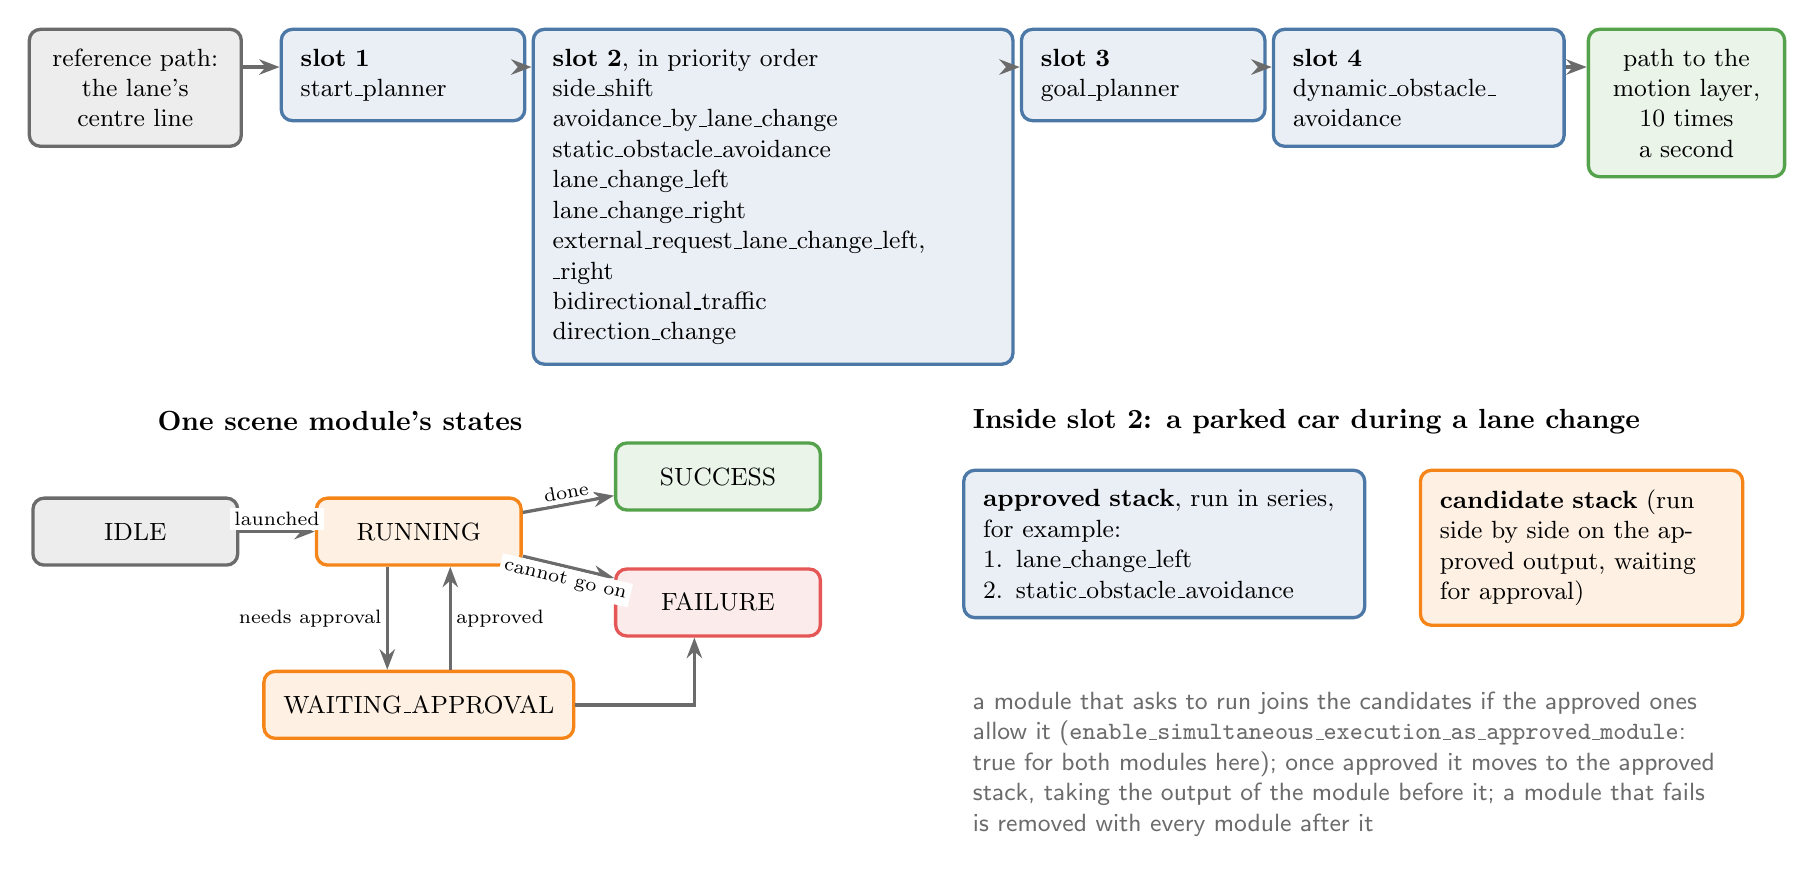
\begin{tikzpicture}[
  slot/.style={box=cblue, font=\small, text width=#1, align=left, minimum height=1.0cm, anchor=north},
  st/.style={box=#1, font=\small, minimum width=2.6cm, minimum height=0.85cm},
  tr/.style={-{Stealth[length=2.6mm]}, draw=cgrey, line width=1.2pt},
  lab/.style={font=\scriptsize, fill=white, inner sep=1.5pt}]
  % the slots
  \node[box=cgrey, font=\small, text width=2.2cm, anchor=north] (ref) at (0,0) {reference path: the lane's centre line};
  \node[slot=2.6cm] (s1) at (3.4,0) {\textbf{slot 1}\\start\_planner};
  \node[slot=5.6cm] (s2) at (8.1,0) {\textbf{slot 2}, in priority order\\side\_shift\\avoidance\_by\_lane\_change\\static\_obstacle\_avoidance\\lane\_change\_left\\lane\_change\_right\\external\_request\_lane\_change\_left, \_right\\bidirectional\_traffic\\direction\_change};
  \node[slot=2.6cm] (s3) at (12.8,0) {\textbf{slot 3}\\goal\_planner};
  \node[slot=3.2cm] (s4) at (16.3,0) {\textbf{slot 4}\\dynamic\_obstacle\_\\avoidance};
  \node[box=cgreen, font=\small, text width=2.0cm, anchor=north] (out) at (19.7,0) {path to the motion layer, 10 times a second};
  \foreach \a/\b in {ref/s1, s1/s2, s2/s3, s3/s4, s4/out} \draw[tr] ([yshift=-0.5cm]\a.north east) -- ([yshift=-0.5cm]\b.north west);
  % a module's states
  \begin{scope}[yshift=-6.4cm]
    \node[font=\bfseries] at (2.6,1.4) {One scene module's states};
    \node[st=cgrey] (idle) at (0,0) {IDLE};
    \node[st=corange] (run) at (3.6,0) {RUNNING};
    \node[st=corange] (wait) at (3.6,-2.2) {WAITING\_APPROVAL};
    \node[st=cgreen] (ok) at (7.4,0.7) {SUCCESS};
    \node[st=cred] (no) at (7.4,-0.9) {FAILURE};
    \draw[tr] (idle) -- node[lab, above] {launched} (run);
    \draw[tr] ([xshift=-4mm]run.south) -- node[lab, left] {needs approval} ([xshift=-4mm]wait.north);
    \draw[tr] ([xshift=4mm]wait.north) -- node[lab, right] {approved} ([xshift=4mm]run.south);
    \draw[tr] (run) -- node[lab, above, sloped] {done} (ok);
    \draw[tr] (run) -- node[lab, below, sloped] {cannot go on} (no);
    \draw[tr] (wait.east) -| ([xshift=-3mm]no.south);
  \end{scope}
  % the two stacks
  \begin{scope}[xshift=10.9cm, yshift=-6.4cm]
    \node[font=\bfseries, anchor=west] at (-0.4,1.4) {Inside slot 2: a parked car during a lane change};
    \node[box=cblue, font=\small, text width=4.6cm, align=left, anchor=north west] (ap) at (-0.4,0.8) {\textbf{approved stack}, run in series, for example:\\1. lane\_change\_left\\2. static\_obstacle\_avoidance};
    \node[box=corange, font=\small, text width=3.6cm, align=left, anchor=north west] (ca) at (5.4,0.8) {\textbf{candidate stack} (run side by side on the approved output, waiting for approval)};
    \node[note, text width=9.6cm, align=left, anchor=north west] at (-0.4,-1.9) {a module that asks to run joins the candidates if the approved ones allow it (\texttt{enable\_simultaneous\_execution\_as\_approved\_module}: true for both modules here); once approved it moves to the approved stack, taking the output of the module before it; a module that fails is removed with every module after it};
  \end{scope}
\end{tikzpicture}
\end{document}
